\chapter{Návrh aplikace}
    Návrh aplikace je velice důležitou součástí projektu pro sjednocení požadavků zadavatelů a reálného provedení. Vytvořením dobrého návrhu se zamezí případným kolizím a zároveň proběhne první interakce mezi zákazníkem a dodavatelem. Pro vzhled aplikace byl ze strany UČL AV vznesen požadavek, aby aplikace byla snadno ovladatelná a měla moderní vzhled. Databázové schéma bylo čistě na našem rozhodnutí a na šifrování uživatelských hesel nebyly vzneseny taktéž žádné požadavky.
    
    

    \section{Wireframy}
        Jednou z nejdůležitějších sekcí bylo navrhnout, jak budou jednotlivé stránky vypadat a kolik jich aplikace bude obsahovat. Základní rozložení stránek bylo na mém rozhodnutí, nicméně musel jsem dodržet požadavky UČL AV. Design měl být jednoduchý, uživatelsky přívětivý a moderní. Tyto návrhy musely být a byly schváleny pracovníky UČL AV. 
        
        Grafika měla být jednoduchá, bez složitých a obsáhlých prvků, proto jsem se rozhodl použít webovou aplikaci Moqups\footnote{domovská stránka: \url{https://moqups.com/}}. Její bezplatná verze nabízí obrovské množství šablon pro grafické návrhy. Od základních prvků jako je tlačítko nebo nadpis, po mírně složitější formuláře nebo dropdowny. Pro snadnější a moderní stylování aplikace jsem chtěl použít Bootstrap, a proto je velikou výhodou, že Moqups má bootstrapovské prvky v nabídce. 
        
        \subsection{Login}
            Pro úvodní přihlašovací stránku jsem vybral jednoducý formulář pro email a heslo viz obrázek \ref{fig:login}. Pro jednoduchost není nutné přidávat další prvky. Pozadí, které by se dalo v budoucím rozšíření změnit, je jako na všech ostatních stránkách bílé.
            
            \begin {figure}[H]\centering
                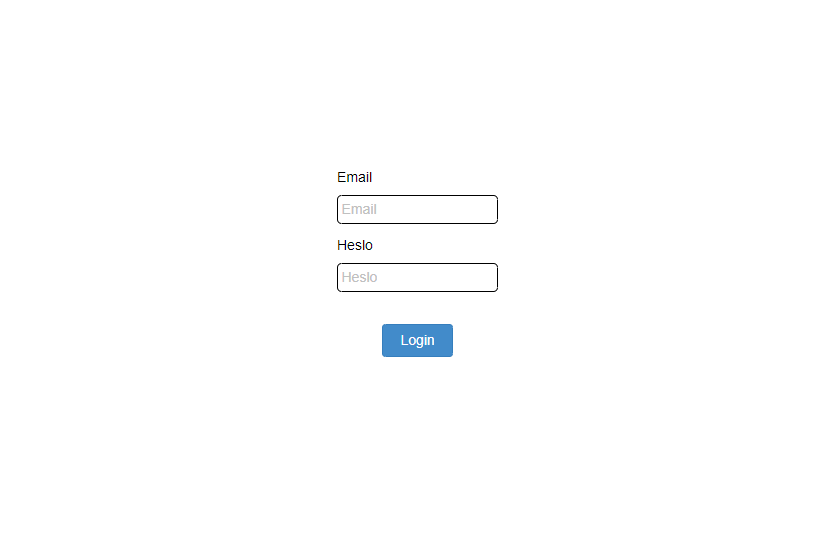
\includegraphics[width=\textwidth]{images/login}
                \caption {Přihlašování}
                \label {fig:login}
            \end{figure}
            
        \subsection{Hlavní stránka}
            Po úspěšném přihlášení do aplikace se zobrazí hlavní stránka, která je rozdělena do tří částí, jak je vidět na obrázku \ref{fig:main}. V hlavičce se nachází odkaz na seznam autorů a vydavatelů děl a dropwdown s možnostmi uživatele. Dále je zde filtr aplikovaný na zobrazená díla. Podle zadání mělo být umožněno vyhledat elektronickou literatutu podle autora, roku vydání, textu obsaženého v díle a podle statusu. Třetí část obsahuje samotný seznam děl, který se dá řadit podle sloupců. U seznamu děl lze nastavit počet zobrazených děl a obsahuje rychlý vyhledávač textu.

        \subsection{Metadata}
            Na obrázku \ref{fig:metadata} je vidět rozložení stránky pro úpravu metadat. Opět se skládá ze tří částí. První hlavička obsahuje navigaci a dropdown pro přihlášeného uživatele. Druhá část je věnována autorům a vydavatelům. V tomto oddílu bude umožněno přidávat a odebírat autora nebo vydavatele. Poslední sekce obsahuje formulář pro úpravu metadat literárního díla. Společně s pracovníky UČL AV byly vybrány nejdůležitější atributy, které je zde možno upravit. 
        
        \subsection{Přílohy}
        
        \subsection{Autoři a vydavatelé}

    \section{Databázové schéma}
        jaké jsem vybral
        
    \section{Autentizace}
        jak je zabezpečené heslo uživatele
